\documentclass[a4paper]{article}

\usepackage{a4wide}
\usepackage{amssymb}
\usepackage{amsthm}
\usepackage{enumitem}
    \setlist[enumerate]{label=(\alph*),itemsep=3pt,topsep=6pt}
    \setlist[itemize]{itemsep=3pt,topsep=6pt}
\usepackage{tikz}
\usepackage[utf8]{inputenc}


\theoremstyle{definition}
\newtheorem{problem}{Příklad}
\newtheorem*{ukol}{Domácí úkol}


\begin{document}

\section*{NAIL062 V\&P Logika: 1. cvičení}


\textbf{Témata:} 
Syntaxe výrokové logiky (strom výrazu, vytvořující strom, prefixový, infixový a postfixový zápis), sémantika výrokové logiky (Booleovské operátory, pravdivostní tabulka, Vennův diagram, tautologie, modely, důsledky). Univerzálnost logických spojek.


\medskip\begin{problem}
Uvažme následující tvrzení:
\begin{itemize}\it
\item Ten, kdo je dobrý běžec a má dobrou kondici, uběhne maraton.
\item Ten, kdo nemá štěstí a nemá dobrou kondici, neuběhne maraton.
\item Ten, kdo uběhne maraton, je dobrý běžec.
\item Budu-li mít štěstí, uběhnu maraton.
\item Mám dobrou kondici.
\end{itemize}
\begin{enumerate}
\item Formalizujte tato tvrzení jako teorii $T$ ve výrokové logice v jazyce $L=\langle b, k, m, s\rangle$, kde výrokové proměnné mají po řadě význam ``být dobrý běžec'', ``mít dobrou kondici'', ``uběhnout maraton'' a ``mít štěstí''.
\item Najděte všechny modely teorie $T$. Pokuste se využít k tomu \emph{tablo}.
\item Napište několik různých důsledků teorie $T$.
\item Najděte CNF teorii ekvivalentní teorii $T$.
\item Výrok je v \emph{disjunktivní normální formě (DNF)}, je-li disjunkcí konjunkcí literálů. Najděte DNF teorii ekvivalentní teorii $T$. 
\end{enumerate}
\end{problem}


\medskip\begin{problem}
Uvažme \emph{vrcholová pokrytí} následujícího grafu:
\begin{center}
    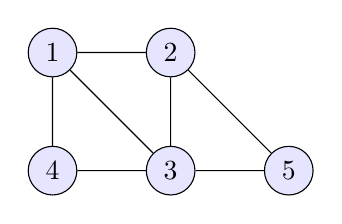
\begin{tikzpicture}[every node/.style={circle,fill=blue!10,draw,minimum size=0.5cm,node distance=1.5cm}]
    \node (1) {$1$};
    \node[right of=1] (2) {$2$};
    \node[below of=2] (3) {$3$};
    \node[left of=3] (4) {$4$};
    \path[draw] (1) -- (2) -- (3) -- (4) -- (1) -- (3);
    \node[right of=3] (5) {$5$};
    \path[draw] (2) -- (5) -- (3);
    \end{tikzpicture}
\end{center}
\begin{enumerate}
    \item Formalizujte ve výrokové logice problém, zda graf na obrázku má nejvýše $k$-prvkové vrcholové pokrytí, pro pevně zvolené $k$. Označme výslednou teorii jako $T_k$.
    \item Ukažte, že $T_2$ nemá žádné modely, tj. graf nemá 2-prvkové vrcholové pokrytí.
    \item Najděte všechna 3-prvková vrcholová pokrytí.
\end{enumerate}
\end{problem}


\medskip\begin{problem}
    Sestrojte strom výrazu (a vytvořující strom), zapište v prefixovém, infixovém a postfixovém formátu:
    \begin{enumerate}
        \item $(3+5)*(-2)+(2*3)$
        \item $(p \to q) \leftrightarrow \neg (p \wedge \neg q)$
        \item $(p \leftrightarrow q) \leftrightarrow ((p \vee q) \to (p \wedge q))$
    \end{enumerate}
\end{problem}


\medskip\begin{problem}
Sestrojte pravdivostní tabulky a Vennův diagram pro následující výrokové formule. Najděte jejich množiny modelů. Které z nich jsou tautologie?\footnote{Venn in doubt, draw a diagram.}
\begin{enumerate}
\item $p \to q \leftrightarrow \neg p \vee q$
\item $(p \to q) \leftrightarrow \neg (p \wedge \neg q)$
\item $((p\to q)\to p)\to p$
\item $\neg (p\vee q)\leftrightarrow \neg p\wedge \neg q$
\end{enumerate}
\end{problem}


\medskip\begin{problem}
    Uveďte příklad výroku v jazyce $\mathbb P=\{p,q,r\}$, který
    \begin{enumerate}
    \item je pravdivý,
    \item je sporný,
    \item je nezávislý,
    \item je ekvivalentní s, ale různý od, výroku $(p\wedge q)\to\neg r$,
    \item má za modely právě $\{(1,0,0),(1,0,1),(0,0,1)\}$.
    \end{enumerate}
\end{problem}


\medskip\begin{problem}
Ukažte, že $\wedge$ a $\vee$ nestačí k definování všech Booleovských operátorů, tj. že $\{\wedge,\vee\}$ není \emph{univerzální} množina logických spojek.
\end{problem}

\medskip\begin{problem} Jsou následující množiny logických spojek univerzální? Zdůvodněte.
\begin{enumerate}
    \item $\{\downarrow\}$ kde $\downarrow$ je Peirce arrow (NOR),
    \item $\{\uparrow\}$ kde $\uparrow$ je Sheffer stroke (NAND),
    \item $\{\vee, \rightarrow, \leftrightarrow\}$,
    \item $\{\vee, \wedge, \rightarrow\}$.
\end{enumerate}
\end{problem}


\medskip\begin{problem}
Uvažte ternární Booleovský operátor $\mathrm{IFTE}(p, q, r)$ definovaný jako ``if $p$ then $q$ else $r$''. 
\begin{enumerate}
    \item Zkonstruujte pravdivostní tabulku.
    \item Ukažte, že všechny základní Booleovské operátory ($\neg, \to, \wedge,\vee,\dots$) lze vyjádřit pomocí IFTE a konstant TRUE a FALSE.
\end{enumerate}  
\end{problem}


\medskip\begin{ukol}[2 body]
{\it Před vypracováním si přečtěte pokyny popsané v podmínkách na zápočet!}
    
\medskip    
    
Adam, Barbora a Cyril jsou vyslýcháni, při jejich výslechu bylo zjištěno následující:
\begin{itemize}\it
    \item Alespoň jeden z vyslýchaných říká pravdu a alespoň jeden lže.
    \item Adam říká: ``Barbora nebo Cyril lžou''
    \item Barbora říká: ``Cyril lže''
    \item Cyril říká: ``Adam nebo Barbora lžou''
\end{itemize}
\begin{enumerate}
    \item Vyjádřete naše znalosti jako výroky $\varphi_1$ až $\varphi_4$ nad množinou prvovýroků $\mathbb{P}=\{a,b,c\}$, přičemž $a,b,c$ znamená (po řadě), že {\it ``Adam/Barbora/Cyril říká pravdu''}.
    \item Najděte všechny modely teorie $T = \{\varphi_1, \dots, \varphi_4\}$.
    \item Najděte CNF teorii ekvivalentní teorii $T$.
    \item Ukažte (libovolnou metodou), že z teorie $T$ plyne, že: {\it Adam říká pravdu.}
\end{enumerate}    
\end{ukol}


\end{document}